\chapter{Design Implementation}

Figure \ref{} shows the earliest high level design of the software for the system created in the first week of the project. At this stage the options were kept open for specific implementation details. The early design essentially required software to be written for three devices; a client computer (GUI), an experiment server (control over access to the system, interface to the GUI, image processing) and an embedded device (controlling experiment hardware). 


Figure \ref{} shows the revised diagram at the time of writing this report. To remove an extra layer of complexity it was decided to use a single device (the BeagleBone Black) to play the role of both the experiment server and the embedded device. From a software perspective, this eliminated the need for an entire layer of communication and synchronization. From a hardware perspective, use of the BeagleBone black instead of a Raspberry Pi removed the need to design or source analogue to digital conversion modules.

Another major design change which occured quite early in the project\footnote{about week 2} is the switch from using multiple processes to running a single multithreaded process on the server. After performing some rudimentary testing it became clear that a system of seperate programs would be difficult to implement and maintain. Threads are similar to processes but are able to directly share memory, with the result that much less synchronisation is required in order to transfer information.

\section{Hardware Interfacing}

Figure \ref{} shows the pin out diagram of the BeagleBone black. There are many contradictory pin out diagrams available on the internet; Figure \ref{} was created by the software team after trial and error testing to determine the correct location of each pin.

The final specification of the pins and functions was chosen by the electrical team, although several earlier specifications were rejected  after difficulties controlling the pins in software. These pins are identified in Table \ref{}.


\subsection{Calibration Methods}

Calibration of the sensors was done at a fairly late stage in the project and only a small number of test points were taken. With the exception of the microscope (discussed in Section \ref{}), all sensors used in this project produce an analogue output. After conditioning and signal processing, this arrives at an analogue input pin on the BeagleBone as a signal in the range $0\to1.8\text{V}$. 


\section{Server Program}


\subsection{Threads and Sampling Rates}

The Server Program runs as a multithreaded process under a POSIX compliant GNU/Linux operating system\footnote{Tested on Debian and Ubuntu}. Each thread runs in parallel and is dedicated to a particular task; the three types of threads we have implemented are:
\begin{enumerate}
  \item Main Thread\ref{} - Starts all other threads, accepts and responds to HTTP requests passed to the program by the HTTP server in the \verb/FastCGI_Loop/ function.
  \item Sensor Thread\ref{} - Each sensor in the system is monitored by an individual thread running the \verb/Sensor_Loop/ function.
  \item Actuator Thread\ref{} - Each actuator in the system is controlled by an individual thread running the \verb/Actuator_Loop/ function.
\end{enumerate}


In reality, threads do not run simultaneously; the operating system is responsible for sharing execution time between threads in the same way as it shares execution times between processes. Because the linux kernel is not deterministic, it is not possible to predict when a given thread is actually running. This renders it impossible to maintain a consistent sampling rate, and necessitates the use of time stamps whenever a data point is recorded. 

Figure \ref{} shows a distribution of times between samples for a test sensor with the software sampling as fast as possible. 
Figure \ref{} shows the distribution when the sampling rate is set to 20Hz. Caution should be taken when interpreting these results, as they rely on the accuracy of timestamps recorded by the same software that is being time sliced by the operating system.

RTLinux is a version of the linux kernel that attempts to increase the predictability of when a process will have control\cite{rtlinux}. It was not possible to obtain a real time linux kernel for the BeagleBone. However, testing on an amd64 laptop (figure \ref{}) showed very little difference in the sampling time distribution when the real time linux kernel was used.





\subsection{Main Thread}

The main thread of the process is responsible for transfering data between the server and the client through the Hypertext Transmission Protocol (HTTP). A library called FastCGI is used to interface with an existing webserver called nginx\cite{nginx}. This configuration and the format of data transferred between the GUI and the server is discussed in more detail Section \ref{}.

Essentially, the main thread of the process responds to HTTP requests. The GUI is designed to send requests periodically (eg: to update a graph) or when a user action is taken (eg: changing the pressure setting). When this is received, the main thread parses the request, the requested action is performed, and a response is sent. The GUI is then responsible for updating its appearance or alerting the user based on this response. Figure \ref{server_overview.png} gives an overview of this process.


\subsection{Sensor Threads}

Figure \ref{sensor_thread.pdf} shows a flow chart for the thread controlling an individual sensor. This process is implemented by \verb/Sensor_Loop/ and associated helper functions.

All sensors are treated as returning a single floating point number when read. A \verb/DataPoint/ consists of a time stamp and the sensor value. \verb/DataPoint/s are continously saved to a binary file as long as the experiment is in process. An appropriate HTTP request (see section\ref{}) will cause the main thread of the server program to respond with \verb/DataPoint/s read back from the file. By using independent threads for reading data and transferring it to the GUI, the system does not rely on maintaining a consistent and synchronised network connection. This means that one the experiment is started with the desired parameters, a user can safely close the GUI or even shutdown their computer without impacting on the operation of the experiment.



As Figure \ref{sensor_thread.pdf} indicates, the processes of actually controlling sensor hardware has been abstracted out of the control loop. A \verb/Sensor/ structure is defined in \verb/sensor.h/ to represent a single sensor. When this structure is initialised, function pointers must be provided; these functions can then be called by \verb/Sensor_Loop/ as needed. All functions related to control over specific sensor hardware can be found in the files within the \verb/sensors/ sub directory.

Earlier versions of the software instead used a \verb/switch/ statement based on the \verb/Sensor/'s id number to determine how to obtain the sensor value. This was found to be difficult to maintain as the number and types of sensors supported by the software were increased.



\subsection{Actuator Threads}

Actuators are controlled by threads in a similar way to sensors. Figure \ref{actuator_thread.pdf} shows a flow chart for these threads. This is implemented in \verb/Actuator_Loop/. Control over real hardware is seperated from the main logic in the same way as sensors (relevant files are in the \verb/actuators/ sub directory). The use of threads to control actuators gives similar advantages in terms of eliminating the need to syncronise the GUI and server software.

The actuator thread has been designed for flexibility in how exactly an actuator is controlled. Rather than specifying a single value, the main thread initialises a structure that determines the behaviour of the actuator over a period of time. The current structure represents a simple set of discrete linear changes in the actuator value. This means that a user does not need to specify every single value for the actuator. The Actuator thread stores a value every time the actuator is changed which can be requested in a similar way to sensor data.



\subsection{Data Storage and Retrieval}

Each sensor or actuator thread stores data points in a seperate binary file identified by the name of the device. When the main thread receives an appropriate HTTP request, it will read data back from the binary file. To allow for selection of a range of data points from the file, a binary search has been implemented.

Several alternate means of data storage were considered for this project. Binary files were chosen because of the significant performance benefit (see Figure \ref{}) and ease with which data can be read from any location in file and converted directly into values. A downside of using binary files is that the server software must always be running in order to convert the data into a human readable format.

\subsection{Authentication}

The \verb/Login_Handler/ function is called in the main thread when a HTTP request for authentication is received. This function checks the user's credentials and will give them access to the system if they are valid.


Whilst we had originally planned to include only a single username and password, changing client requirements forced us to investigate many alternative authentication methods to cope with multiple users.

Several authentication methods are supported by the server; the method to use can be specified as an argument when the server is started.
\begin{enumerate}
  \item {\bf Unix style authentication}


  Unix like operating systems store a plain text file (/etc/shadow) of usernames and encrypted passwords. To check a password is valid, it is encrypted and then compared to the stored encrypted password. The actual password is never stored anywhere. The /etc/shadow file must be maintained by shell commands run directly from the beaglebone. Alternatively a web based system to upload a similar file may be created.

  \item {\bf Lightweight Directory Access Protocol (LDAP)}

  LDAP is a widely used data base for storing user information. A central server is required to maintain the LDAP database; programs running on the same network can query the server for authentication purposes.

  The UWA user management system (pheme) employs an LDAP server for storing user information and passwords. The software has been designed so that it can interface with an LDAP server configured similarly to the server on UWA's network. Unfortunately we were unable to gain permission to query this server. However an alternative server could be setup to provide this authentication mechanism for our system.


  \item {\bf MySQL Database}

	MySQL is a popular and free database system that is widely used in web applications. The ability to search for a user in a MySQL database and check their encrypted password was added late in the design as an alternative to LDAP. There are several existing online user management systems which interface with a MySQL database, and so it is feasable to employ one of these to maintain a list of users authorised to access the experiment. UserCake is recommended, as it is both minimalistic and open source, so can be modified to suit future requirements.


  MySQL and other databases are vulnerable to many different security issues which we did not have sufficient time to fully explore. Care should be taken to ensure that all these issues are addressed before deploying the system.



\end{enumerate}

\subsection{Safety Mechanisms}

Given the inexperienced nature of the software team, the limited development time, and the unclear specifications, it is not wise to trust safety aspects of the system to software alone. It should also be mentioned that the correct functioning of the system is reliant not only upon the software written during this project, but also the many libraries which are used, and the operating system under which it runs. We found during development that many of the mechanisms for controlling BeagleBone hardware are unreliable and have unresolved issues. We attempted to incorporate safety mechanisms into the software wherever possible.

Sensors and Actuators should define an initialisation and cleanup function. For an actuator (eg: the pressure regulator), the cleanup function must set the actuator to a predefined safe value (in the case of pressure, atmospheric pressure) before it can be deinitialised. In the case of a software error or user defined emergency, the \verb/Fatal/ function can be called from any point in the software; this will lead to the cleanup functions of devices being called, which will in turn lead to the pressure being set to a safe value. The cleanup functions will also be called if the software exits unexpectedly.

Sensors and Actuators are designed to include a \verb/sanity/ function which will check a reading or setting is safe respectively. These checks occur whenever a sensor value is read or an actuator is about to be set. In the case of a sensor reading failing the sanity check, \verb/Fatal/ is called immediately and the software shuts down the experiment. In the case of an actuator being set to an unsafe value the software will simply refuse to set the value.


\subsection{Performance}

Figure \ref{} shows the CPU and memory usage of the server program with different numbers of dummy sensor threads. This gives an idea of how well the system would scale if all sensors were run on the same BeagleBone.

\begin{figure}[H]
	\centering
	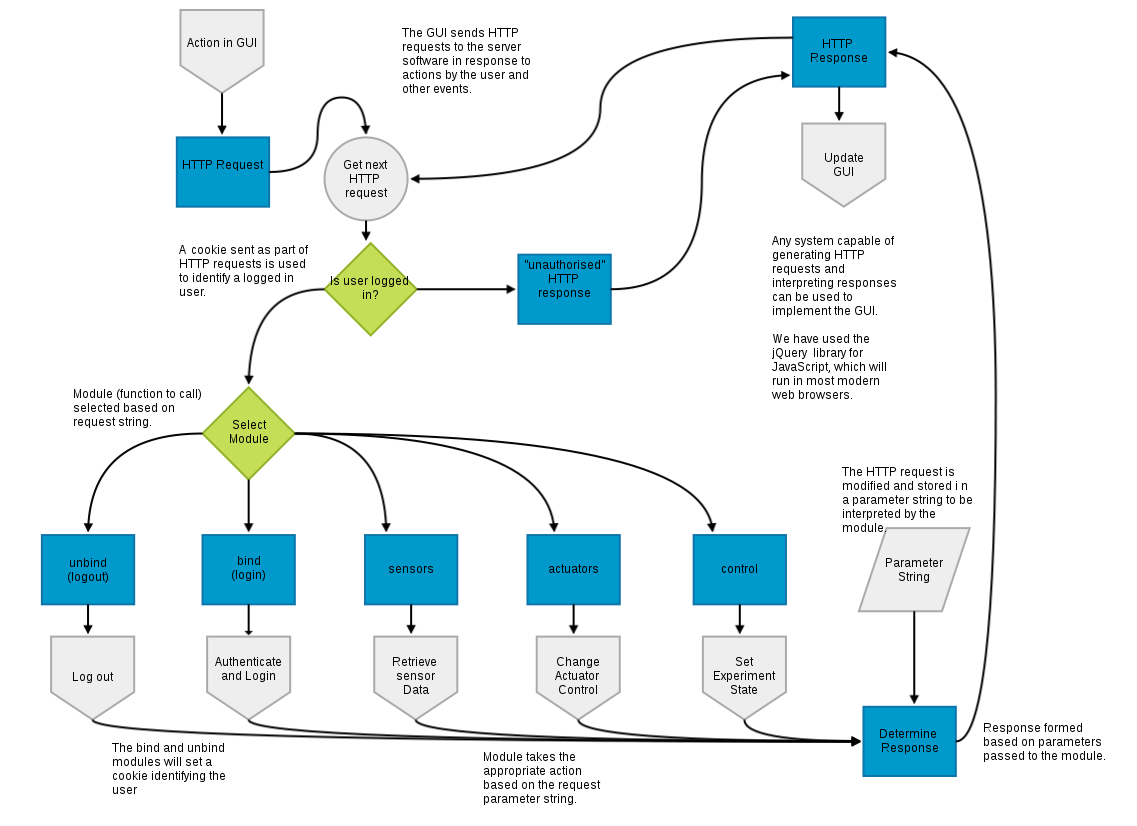
\includegraphics[width=1.0\textwidth]{figures/server_overview.png}
	\caption{Server overview} 
	\label{server_overview.png}
\end{figure}


\pagebreak
\begin{figure}[H]
	\centering
	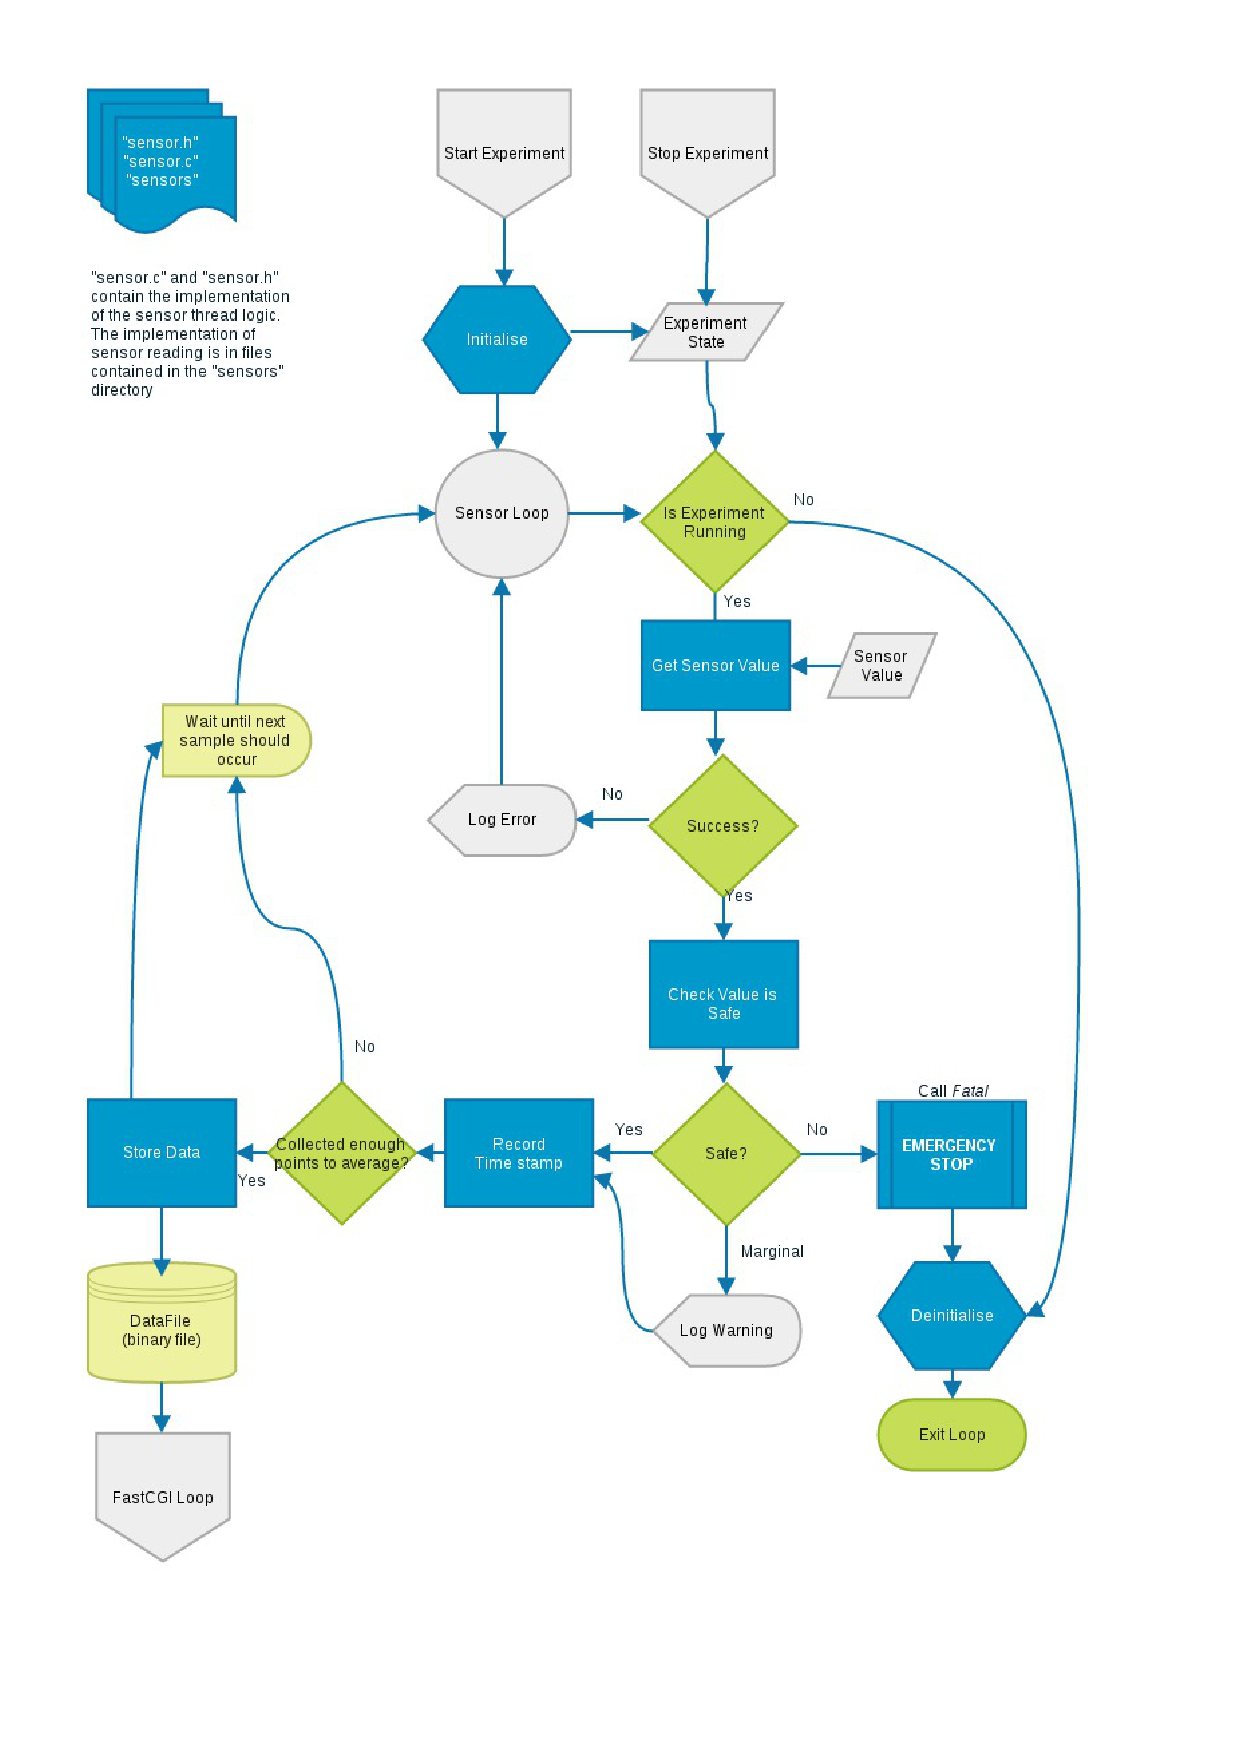
\includegraphics[width=1.1\textwidth]{figures/sensor_thread.pdf}
	\caption{Flow chart for a sensor thread} 
	\label{sensor_thread.pdf}
\end{figure}
\pagebreak
\pagebreak
\begin{figure}[H]
	\centering
	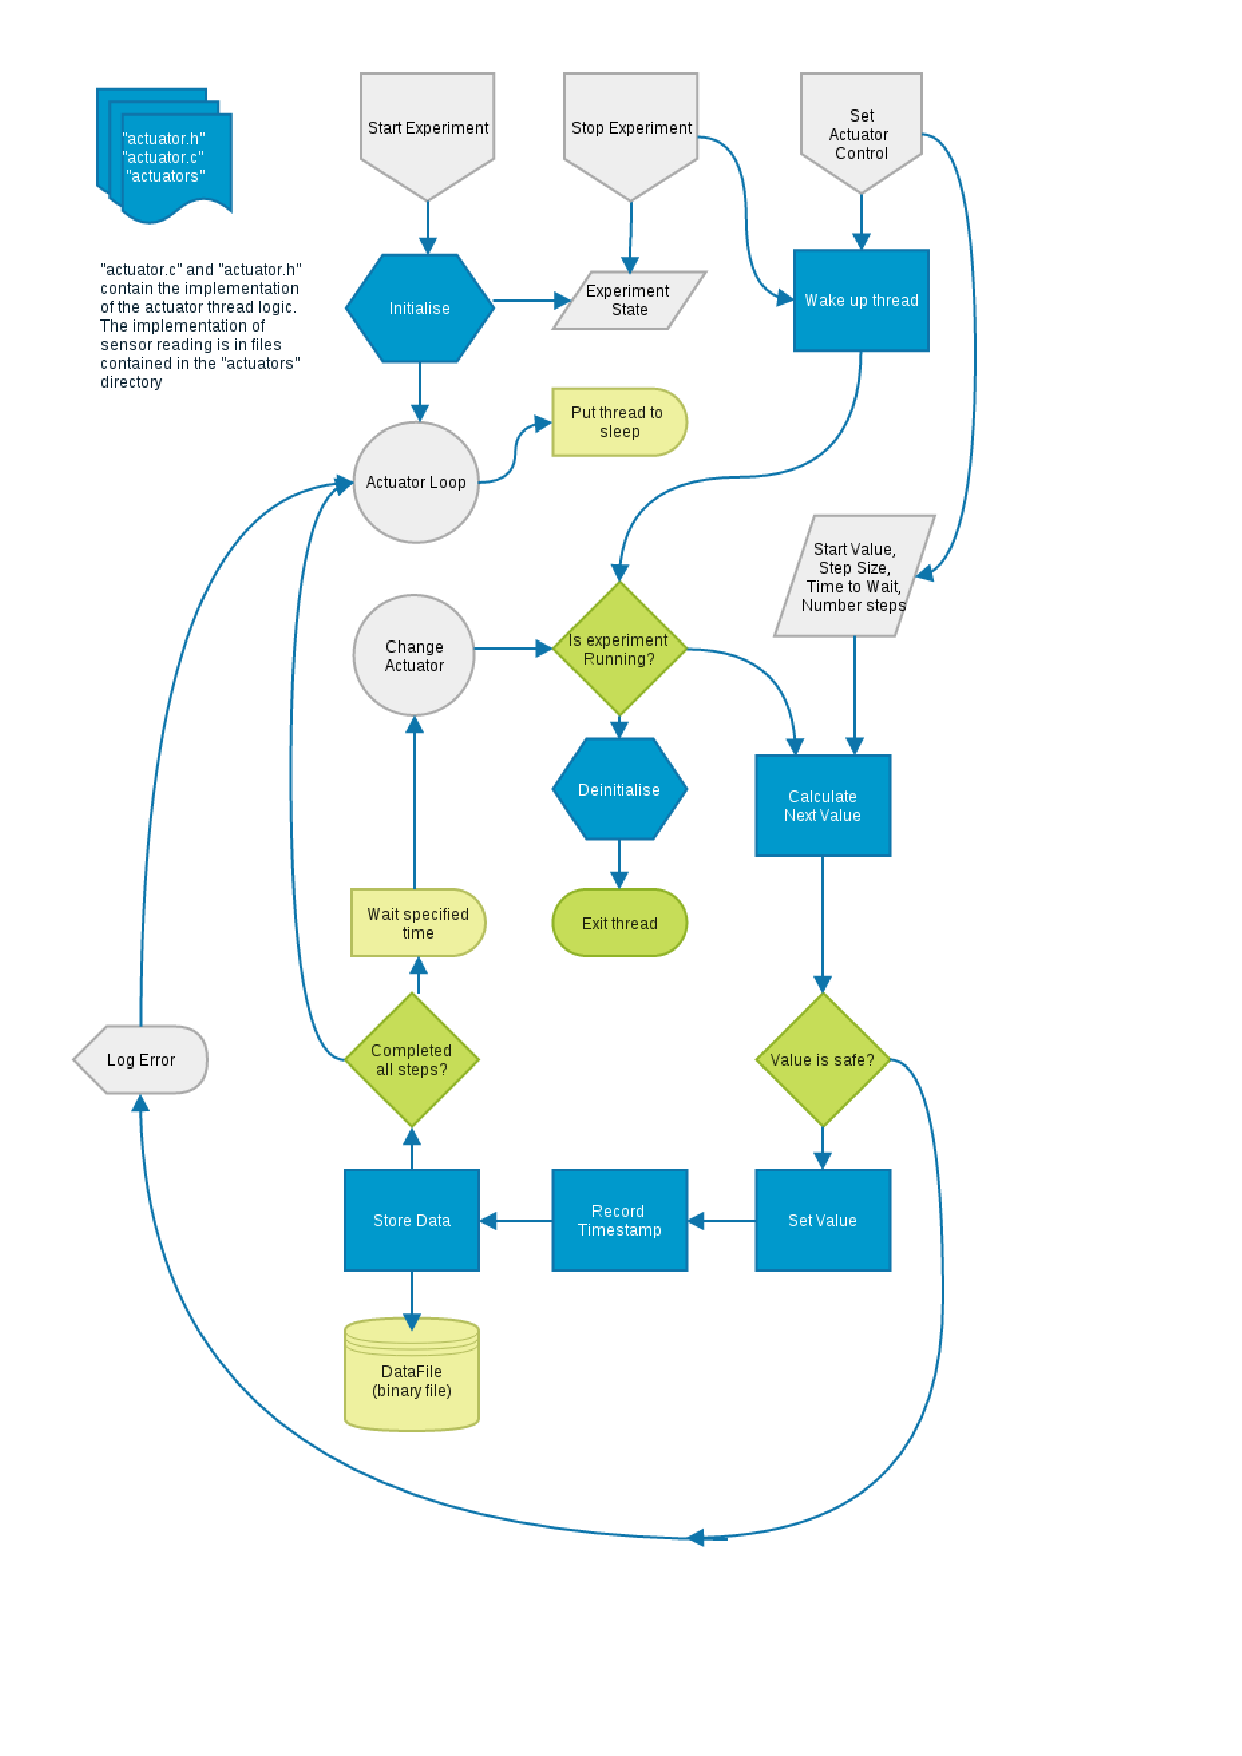
\includegraphics[width=1.1\textwidth]{figures/actuator_thread.pdf}
	\caption{Flow chart for an actuator thread} 
	\label{actuator_thread.pdf}
\end{figure}
\pagebreak

\section{Image Processing}

\section{Client Program}



\subsection{Human Computer Interaction}

\subsection{Interaction with API}









